\documentclass[journal]{IEEEtran}
\usepackage{blindtext}
\usepackage{graphicx}
\usepackage{url}
\usepackage{amsmath,amssymb}

\begin{document}
\title{Click-Through Rate Prediction for Sponsored Search Advertising in Microsofts Bing Search Engine}
\author{Craig Heptinstall Crh13- 110005643 \\
SEM6120\\Institute of Computer Science\\Aberystywth University}

\maketitle


\begin{abstract}
In 2009, a paper by Thor Graepel \cite{bing-paper} described a winning click-through rate (CTR) prediction algorithm used for sponsored search in Microsoft's Bing search engine (the authors named this adPredictor). The paper introduced a Bayesian online learning concept that was chosen to replace the previous CTR algorithm. Here this paper looks at the concepts used in the adPredictor algorithm and how appropriate certain aspects of the task were identified and dealt with. Following an evaluation of the algorithm and paper itself, there are of course, always further improvements possible to any algorithm. Using other research, suggestions have been presented to increase the efficiency of the solution, especially over the web (since this algorithm should work efficiently during real time searches).

\end{abstract}

\section{Sponsored search}
Sponsored search is considered as one of the most profitable business models today, and according to several sources of analytic services such as analytics-magazine \cite{business-model} the four top search engines(Bing, Google, Yahoo and Baidu) make in excel of \$37 billion. Bing however gets the lion share with over \$25 billion of the total coming its own way. Therefore, keeping this amount on an upward trend requires appropriate and efficient advertisements. \\
Sponsored search uses two key aspects to the use of a search engine that can be applied to providing advertisements:
\begin{itemize}
\item The query the users enter- This indicates the requirement of the user
\item Users clicking on advertisements- This gives users the opportunity to see advertiser's pages
\end{itemize}
In order to get the advertisements that is useful to the search engine (in terms of revenue), the advertisers (in terms of clicks on their links), and user's needs (In terms of relevant adverts), CTR prediction is a most vital part of a search engine.

\subsection{Click rate prediction}
The paper begins by detailing what click rate prediction is and how it fits into the web framework that is the Bing search engine. Getting an accurate metric for where advertisements will be clicked is important to the user, and more so the search engine. By being able to get the probability of an advert being clicked, the authors are able to increase further the possible profitability of the search engine via advert placement, and assisting the choice of adverts to be displayed. \\
Although the paper describes CTR well as a starting point, the graph in figure \ref{fig:CTR} shows an example of how keywords and where they are placed on a page affect the CTR. By having a good predictor, the keywords and placement of adverts will be more informed before they are added to search.

\begin{figure}[!ht]
  \caption{CTR based on position of advertisement. Image taken from a marketing explanation of CTR \cite{ctr-image}.}
  \centering
  \label{fig:CTR}
    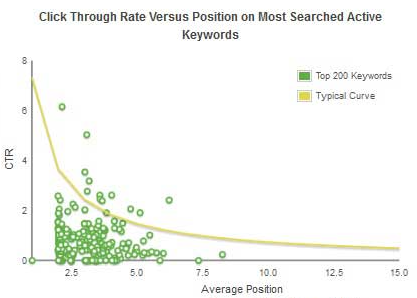
\includegraphics[width=0.5\textwidth]{CTR}
\end{figure}

\subsection{Keywords auction}
In order to grasp the whole concept of CTR prediction, keyword auction is something that the paper describes as an important feature in displaying advertisements in their specific places. Rather than having selected ads chosen by the selecting algorithm just place them in any order on the screen, keyword auction uses an algorithm known as generalized second price (GSP). This ensures that advertisers pay appropriate amounts referring to what position they appear on a search page. \\
GSP is a fairly simple algorithm \cite{keyword-auction}, which takes in a number of bids from bidders (in this case advertisers) all of which specify amounts they are willing to pay for clicks on adverts related to certain keywords. Following the auction, the bids with the highest prices win the best place, but only pay the second highest bid price. After this, the second highest pays the second highest bid and so on. Predicting which advertisements will be used by users heavily relies on the results from a GSP, which the adPredictor paper expands on with constraints that this way of generating advertisements brings.

\section{Challenges approached by adPredictor}
There were a number of existing problems that needed to be solved by any CTR predictor in order to create an efficient solution that would be enough to replace Bing's previous predictor. These range from getting suitable input features for the predictor, to evaluating the performance of the predictor itself. This section of the paper looks at each of these in relation to what the adPredictor authors had to accomplish in order for their solution to work.

\subsection{Features and impressions}
With any machine learning algorithm, there must be appropriate input features that can represent variables used to produce outcomes (in this case binary). Because the web is quite diverse, and is forever changing, many different aspects of a user's actions should be considered when predicting click through rates. The authors of adPredictor questions the availability of inputs, and comes to a conclusion that at least three main categories should be considered when attempting to create the probability of a user's click:
\begin{enumerate}
\item Ad features- The adverts themselves, including links, text on the adverts and the campaign of the ad.
\item Query features- These are directly entered by the user, such as words searched by the user.
\item Context features- Indirectly given by the user, to personalise adverts more. These could be the location of the user, time and date to name a few.
\end{enumerate}
Because of the vast size features possible, the complexity of the algorithm had to be considered, alongside the speed of which the predictor would function. Selecting good features is one of the building blocks of any machine learning algorithm. In a lecture by Jeff Howbert at Washington University \cite{washington}, he mentions the 'Curse of dimensionality' and states that as features increase the volume of feature space increases too. This makes data harder to understand and results in an increase of difficulty of achieving statistical significances.

\subsection{Isolated predictions}
The next task challenging the authors was the testing of the predictor. In order to actually see results from their algorithm, there was the task of seeing how well it performed. Although the author suggests a number of ways that machine learning predictors can be tested (AUC (area under the receiver operator curve), or log-likelihood of test data), with the predictor being part of a larger system means that different goals from users, advertisers and the search engine may conflict resulting in inaccurate test results.

\subsection{Dynamic web}
Another challenge identified in the paper looks at the dynamic behaviour of the web. Because the web is not a static object, the ways people use it will vary over time. The authors also highlight such times as seasonal changes, changes in viral interest and economic behaviours that can all change the way the general interest of different searches head. Following this, the CTR predictor must be able to cope with changes in clicks for certain topics. Because the current ad-selection technique (keyword auction) only bases its choices from advertisers who will update their target markets, it means that long term click through rates will be ignored, whilst the algorithm used in a predictor would still be trying to base its predictions from learning with older data.

\subsection{Computational issues}
A final issue identified by the authors, and generally across wide research into CTR predictors is the worry of computational power. With the scale of the web being so large, the amount of advertisements and their data can be extremely large. With each search having to calculate and bring back the most appropriate advertisements almost instantaneously, the algorithm defined in the resulting paper had to be as efficient as possible. \\
Training of the algorithm must also be performed as quickly as possible to keep up with the changing trends of a web platform. There is a trade-off between accuracy and computing time that had to be considered. A paper that looked at a similar system created for Facebook advertisements \cite{facebook} highlights the importance of 'keeping memory and latency contained for massive scale'. The creators of adPredictor would also have had to ensure that as much data could be used as features, while keeping the speed of the predictor at a sufficient level.

\section{adPredictor solution}
For the solution presented in the paper, the authors chose to start with a general Bayesian online learning algorithm, and then mutated this to work with CTR terminology. The image below \ref{fig:bayes} indicates the general use Of Bayes rule, where in this case the posterior being the binary outcome of whether the user would or would not click the advertisement. \\

\begin{figure}[!ht]
  \caption{General Bayes rule, where \(P(h \mid d)\) is the binary probability of clicking an advertisement}
  \centering
  \label{fig:bayes}
    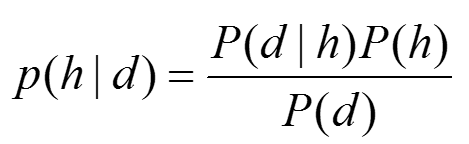
\includegraphics[width=0.3\textwidth]{bayes}
\end{figure}

The algorithm bases itself off a probit regression model that takes in features (in this case the three categories mentioned earlier: ad, query and context features), and performs online Gaussian updates to the model created. Continuing from that to suit it more towards the use of online CTR prediction, pruning of some common features are performed to cut the training time of the algorithm. Finally, the algorithm uses parallel training to ensure that new data from the ever-changing web are taken into account, avoiding solely building on already existing static data. \\
Notating the outputs of the algorithm was the first step in the adPredictor algorithm, and the authors made it so a simple vector would hold a range of feature values for an advertisement, and where the outcome of a click/ none click will be represented by 1 or -1 for notational convenience. 
The probability model the authors decided to use was a generalised linear model with a probit link function. From comparison of this with a standard linear model, there could be two reasons for this use (both of which can be also explained in textbook found about GLM’s from Dell \cite{dell}):
\begin{enumerate}
\item Distribution of dependent variable- The dependent variable (in this case click rates) may not be continuous in a linear distribution.
\item None-linear effect of prediction- The effect of the predictor will not be linear, because the nature of clicks by users will not be concrete.
\end{enumerate}
At this point, Gaussian prior distribution is applied over the weights of the model, in order to take into account previous click estimations. The paper represents this in a factor graph model, showing how the probit regression function works. The model takes in Gaussian prior weights, calculates a score for each, and then compares a zero-mean Gaussian of the weight with a given threshold. \\
The paper talks about the use of 'update equations' which allow the algorithm to become more a natural online learning means, taking into account any prior information (such as historical average CTR). The possible issue here (as mentioned in section 2.C) is that with the dynamics of the web, historical averages may not be sufficient in the learning of the algorithm. \\
Continuing on with the need for a solution to web dynamics, the algorithm then puts in place a model of dynamics that converges back to the prior rather than to a uniform distribution of weights. By delaying updates of weights, computationally it makes it possible to apply updates cumulatively resulting in the allowance of new data. \\
Another important aspect of the solution proposed in the paper looks more towards the computational costs of the algorithm when placing it in a web environment. As identified in the potential issues from the previous section, the memory and data size footprint must be limited in order to allow this algorithm to be deployed for its intended function. By compressing the model to only concentrate on features that appear commonly (though new features should be considered in case they become a new common), the model will not waste memory on them. \\
Training and feedback of the usefulness of the algorithm is 


\subsection{Solution issues}
\section{Suggested alternatives}
\section{Evaluation}
\subsection{Future developments}

\appendices

\ifCLASSOPTIONcaptionsoff
  \newpage
\fi

\begin{thebibliography}{1}

\bibitem{bing-paper}
T.~Graepel, \emph{Web-Scale Bayesian Click-Through Rate Prediction for Sponsored Search Advertising in Microsoft's Bing Search Engine}, \hskip 1em plus
  0.5em minus 0.4em\relax Microsoft Research Ltd, 2010.
  
\bibitem{business-model}
P.~Quinn, \emph{Sponsored search advertising}, \hskip 1em plus
  0.5em minus 0.4em\relax Analytics Magazine, \emph{\url{http://www.analytics-magazine.org/may-june-2012/580-online-analytics-sponsored-search-advertising}}, 2012.
  
\bibitem{keyword-auction}
B.~Edelman, \emph{Internet Advertising and the Generalized Second-Price Auction:
Selling Billions of Dollars Worth of Keywords}, \hskip 1em plus
  0.5em minus 0.4em\relax \url{www.benedelman.org}, 2006.
  
\bibitem{ctr-image}
L.~Kim, \emph{Five Must-Have Insights for Better PPC Campaign Performance}, \hskip 1em plus
  0.5em minus 0.4em\relax Marketing Profs, \emph{\url{http://www.marketingprofs.com/articles/2014/24562/five-must-have-insights-for-better-ppc-campaign-performance}}, 2014.
  
\bibitem{washington}
J.~Howbert, \emph{Machine Learning: Feature Creation and Selection
}, \hskip 1em plus
  0.5em minus 0.4em\relax \url{http://courses.washington.edu}, 2012.
  
\bibitem{facebook}
X.~He, \emph{Practical Lessons from Predicting Clicks on Ads at Facebook}, \hskip 1em plus
  0.5em minus 0.4em\relax \url{https://research.facebook.com/publications/practical-lessons-from-predicting-clicks-on-ads-at-facebook/}, 2014.
 
\bibitem{dell}
Dell.Inc, \emph{Generalized Linear Models}, \hskip 1em plus
  0.5em minus 0.4em\relax Marketing Profs, \emph{\url{http://documents.software.dell.com/Statistics/Textbook/Generalized-Linear-Models}}, 2015.
  
\end{thebibliography}

\end{document}